\documentclass[12pt,a4paper]{article}
\usepackage[width=.75\textwidth]{caption}
\usepackage{graphicx}
\usepackage{authblk}
\usepackage{amsmath}
\usepackage{amsfonts}
\usepackage{braket}
\usepackage{epigraph}
%\usepackage{mathrsfs}
\usepackage[mathscr]{euscript}
\usepackage[top=2cm, bottom=2cm, left=2cm, right=2cm]{geometry}
\usepackage{fancyhdr}

\setlength{\epigraphwidth}{0.8\textwidth}

% \pagestyle{fancy}
\begin{document}

%title and author details
\title{Emergent Spacetime from Matter Emanations}
\author[1]{Kevin Player\footnote{kplayer@andrew.cmu.edu}}

\maketitle

\epigraph{Quote}{Quoter}



\abstract{Einstein taught us that matter does not merely traverse spacetime passively; it actively shapes and warps the spacetime it occupies. Expanding on this idea, we investigate how De Broglie matter waves can be employed to construct an emergent spacetime, realizing spacetime as an inherent property of the matter itself. Throughout this exploration, we uncover various connections to quantum gravity.}
 
\section{Counting Ticks for Emergent Time}

Recall that a massive particle with mass $m$, such as an electron, has a DeBroglie frequency $\omega = mc^2 / h$. We will discuss the number of ``ticks'' (at frequency $\omega$) that the particle has undergone. In this context, $\omega$ functions like a sampling rate for the matter in ticks per second, much like Bremermann's limit.  We treat this number as a quantum observable.  It will serve as an emergent measure of (proper) time for the particle.  In this way events on a time line make sense as a property of the particle; we count them as the number of ticks, or the number of zero phase crossings of the complex matter wave.

\section{Double Slit for Emergent Space}


\begin{figure}[h!]
\centering
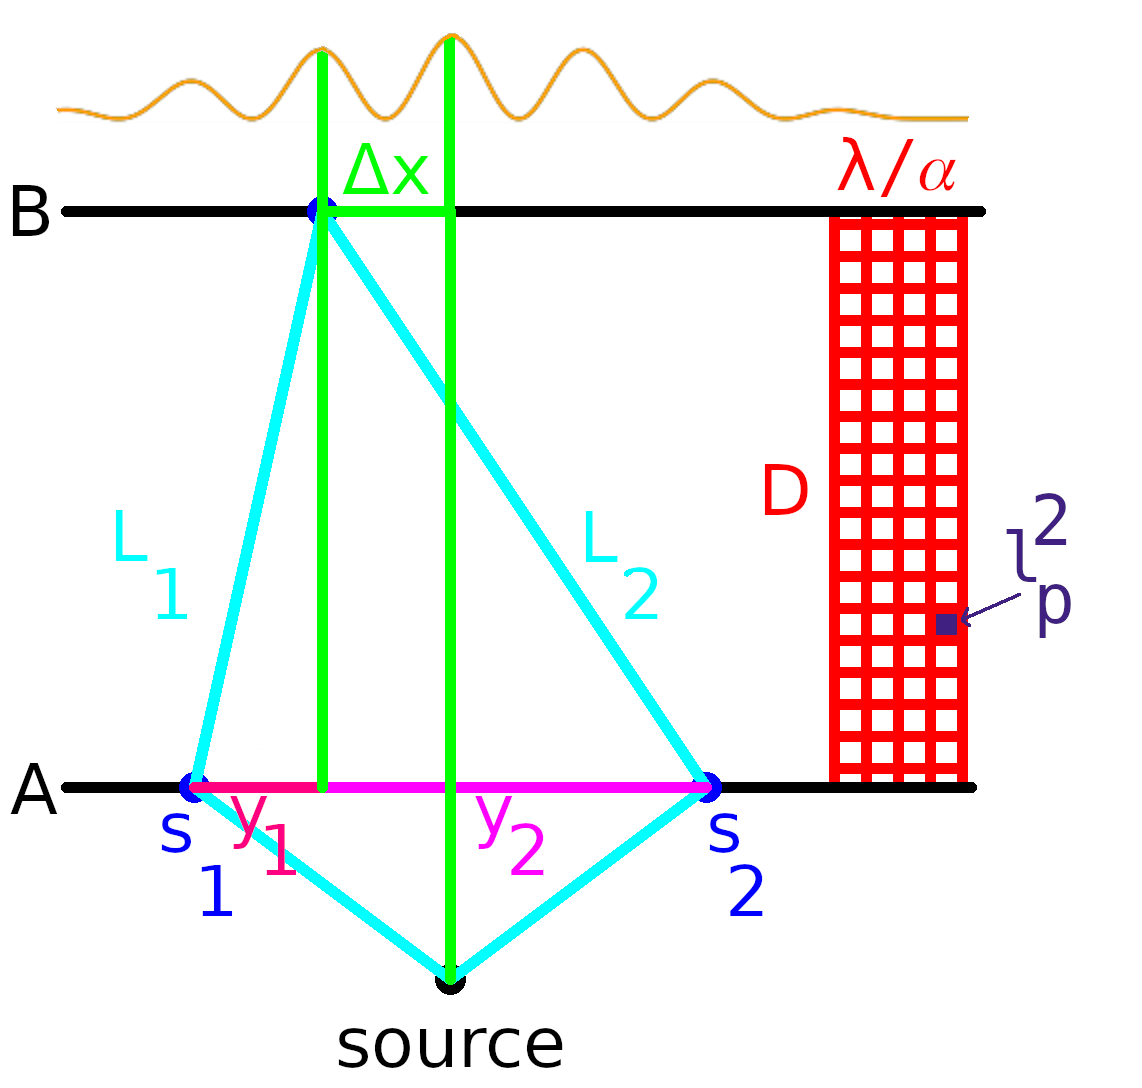
\includegraphics[scale=0.5]{double_slit.png}
\caption{Typical Double Slit Setup.  $D$ is the distance between screens $A$ and $B$. $\Delta s$ is the distance between slits.  $\Delta x$ is the distance between fringes. $\Delta L = \lambda$ is the difference of path lengths.  $\frac{\lambda D}{\alpha^2}$ is shown to be made up of Planck length squares.}
\label{screen}
\end{figure}


Next consider the situation in Figure \ref{screen}.  The particle of mass $m$ is in quantum superposition, going through two slits, $s_1$ and $s_2$, on a one dimensional screen $A$. Let B be another screen behind $A$ with distance $D$ between them. Then for any time $t$ and position $x$, causally beyond $s_1$ and $s_2$, we have the number of ticks $n_1$ with repect to $s_1$ and $n_2$ with repect to $s_2$. So $(n_1,n_2)$ is a function of $(t,x)$. Note that the interference patterns that appear on a screen $B$ are given by fringes each of which can be labeled by a unique $n_2 - n_1$. We will use this to describe a way in which space emerges as a property of the massive particle. 

Let $L_1$ and $L_2$ be the lengths of the path from the source to the screen for the particle going through $s_1$ and $s_2$ respectively. Let the particle have a wavelength of $\lambda = \Delta L$ and we consider the first noncentral fringe at distance $\Delta x$ away from the center.  We have $L_i = \sqrt{y_i^2 + D^2}$ and approximating the square root we have $\lambda \approx \frac{\Delta s \Delta x}{D}$.

Consider the local behaviour of the interference pattern near the middle of $B$ (the central fringe). The fringe pattern is locally made up of a combination of a part in space (fringes) and a part in time (evolution). Let $n_{1,2} = (n_1, n_2)$ label the antinodes of this pattern in space-time. The antinodes each pick out individual $n_{1,2}$ values, associated with the zero phase. We can write out a 2d joint frequency $\nu = \omega * \omega$ (in Hz * Hz) of this pattern using $\Delta x$ and $\Delta t$.  Using the energy of the particle $E_h = h \omega = \frac{h}{\Delta t}$, we have
\begin{equation}
\label{nu_h}
  \nu = \frac{c}{\Delta x \Delta t} = \frac{c}{h \lambda D} E_h \Delta{s}
\end{equation}
where we have
\begin{equation}
\label{def_h}
E_h = m c^2
\end{equation}


Let $\Delta(s) = s_2 - s_1$ and let $E_G$ be the gravitational (self) energy of the particle
\begin{equation}
\label{def_G}
E_G = \frac{G m^2}{\Delta s}
\end{equation}
Using the gravitational potential and setting $m^2$  equal to $w^2$ times the squared Bremermann constant $c^4/h^2$ we have
\begin{equation}
\label{nu_G}
\nu = \omega^2 = \frac{c^4}{G h^2} E_G \Delta s
\end{equation}


We have written $\nu$ in two ways, equations (\ref{nu_h}) and (\ref{nu_G}). Setting these two representations of $\nu$ equal to each other we get
\[
\lambda D = \frac{E_h}{E_G} l_p^2 = (\alpha l_p)^2
\]
where $l_p$ is the Planck length and we define $\alpha = \sqrt{\frac{E_h}{E_G}}$. This suggestively counts Planck areas in $\lambda D$ scaled by the unitless $\alpha$.
\[
   N = \frac{\lambda D}{(\alpha l_p)^2}
\]
In fact we have another way of understanding $\alpha$.  By using equatios (\ref{def_h}) and (\ref{def_G}) we have
\[
  \frac{1}{\alpha^2} = \frac{E_G}{E_h} = \frac{Gm}{c^2\Delta s} = \left(\frac{v_e}{c}\right)^2
\]
where $v_e$ is an escape velocity.  With this understanding we must have
\[
   E_h \ge E_g
\]
with equality if and only if $v_e = c$, that is if and only if the particle is a black hole.  In this case the suggestive $N$ is the count of plack areas $l_p^2$ from black hole thermodynamics where an event horizon is equal to $\lambda D$. The treatment in this note gives us a construct for the less exotic case $v_e < v$.


\end{document}
